\documentclass[a4paper, 12pt]{article}
\usepackage[utf8]{inputenc}
\usepackage[english,russian]{babel}
\usepackage[warn]{mathtext}
\usepackage{graphicx}
\usepackage{float}
\usepackage{multirow}
\restylefloat{table}
\usepackage{amsmath}
\usepackage{floatflt}
\usepackage[T2A]{fontenc}
\usepackage[left=20mm, top=20mm, right=20mm, bottom=20mm, footskip=10mm]{geometry}

\tolerance 1414
\hbadness 1414
\emergencystretch 1.5em
\hfuzz 0.3pt        % размер максимального переполнения без warning'a
\widowpenalty=10000 % запрещает одиночную строку абзаца в начале страницы
\vfuzz \hfuzz
\raggedbottom       % если на странице мало содержимого, добавить пустое место в конце, а не в середине страницы



\begin{document}

\begin{titlepage}
	\centering
	\vspace{5cm}
	{\scshape\LARGE московский физико-технический институт (национальный исследовательский университет) \par}
	\vspace{6cm}
	{\scshape\Large Лабораторная работа 4.2 \par}
	{\huge\bfseries Исследование энергетического спектра $\beta$-частиц \par}
	\vspace{1cm}
	\vfill
\begin{flushright}
	{\large Б03-104}\par
	\vspace{0.3cm}
	{\LARGE Куланов Александр}
\end{flushright}
	

	\vfill


	Долгопрудный, 2023 г.
\end{titlepage}

\begin{itemize}
	\item \textbf{Цель работы:} с помощью магнитного спектрометра исследовать энергетический спектр $\beta$-частиц при распаде ядер $^{137}$Cs и определить их максимальную энергию.
\end{itemize}

\section{Теоретические сведения}
Бета-распадом называется самопроизвольное превращение ядер, при котором их массовое число не изменяется, а заряд увеличивается или уменьшается на единицу. Бета-активные ядра встречаются во всей области значений массового числа $A$, начиная от единицы (свободный нейтрон) и кончая самыми тяжелыми ядрами. Период полураспада $\beta$-активных ядер изменяется от ничтожных долей секунды до $10^{18}$ лет. Выделяющаяся при единичном акте $\beta$-распада энергия варьируется от 18 кэВ (для распада трития ${ }_1^3 \mathrm{H}$ ) до 13,4 МэВ (для распада изотопа бора ${ }_5^{12} \mathrm{~B}$.)
В данной работе мы будем иметь дело с электронным распадом
\begin{equation*}
{ }_{\mathrm{Z}}^A \mathrm{X} \rightarrow{ }_{\mathrm{Z}+1}^A \mathrm{X}+e^{-}+\tilde{v},
\end{equation*}

при котором кроме электрона испускается антинейтрино. Освобождающаяся при $\beta$-распаде энергия делится между электроном, антинейтрино и дочерним ядром, однако доля энергии, передаваемой ядру, исчезающе мала по сравнению с энергией, уносимой электроном и антинейтрино. Практически можно считать, что эти две частицы делят между собой всю освобождающуюся энергию. Поэтому электроны могут иметь любое значение энергии - от нулевой до некоторой максимальной, которая равна энергии, освобождающейся при $\beta$-распаде, и является важной физической величиной.

\begin{figure}[H]
    \centering
    \includegraphics[width=0.7\textwidth]{graph1.png}
    \caption{Форма спектра $\beta$-частиц}
    \label{fig:plot1}
\end{figure}

Вид спектра $\beta$-частиц показан на рис. 1. Величина $W\left(p_e\right) d p_e$ oпределяет вероятность того, что $\beta$-частица получит при испускании импульс, лежащий в интервале от $p_e$ до $p_e+d p_e$. Величина $W\left(p_e\right)$ является плотностью вероятности, т. е. вероятностью, отнесенной к единичному интервалу импульсов. Распределение электронов по энергии (или по импульсу) может быть вычислено тсоретически. Для разрешенных переходов) вероятность $\beta$-распада просто пропорциональна статистическому весу, т. е. фазовому объему в векторном пространстве импульсов электронов и нейтрино.

Рассмотрим сначала систему отсчета в трехмерном пространстве, осями которой являются проекции импульса электрона. Интервалу от $p_c$ до $p_e+d p_c$ соответствует в таком пространстве шаровой слой с радиусом $p_c$ и шириной $d p_c$. Объем этого слоя равен $4 \pi p_e^2 d p_c$. Импульс электрона определяет его энергию. Сумма энергий электрона и антинейтрино практически равна энергии распада, и поэтому задание импульса электрона $p_c$ определяет энергию, уносимую антинейтрино, а вместе с ней и абсолютную величину его импульса. Направление импульса антинейтрино остается свободным. В пространстве импульсов, уносимых антинейтрино, выделяется, таким образом, шаровой слой площадью $4 \pi p_v^2$. Имеем поэтому
\begin{equation}
W\left(p_e\right) d p_e \propto p_e^2 p_v^2 d p_e .
\end{equation}

Выразим в этом соотношении $p_v$ через $p_e$. Масса антинейтрино равна нуло. Следовательно,
\begin{equation}
p_v=E_v / c=\left(T_{\max }-T_c\right) / c .
\end{equation}

В этом уравнении $E_v-$ кинетичсская энергия антинейтрино (совпадающая с его полной энергией), $T_{\max }-$ максимально возможная в данном распаде кинетическая энергия электрона, $T_e-$ его фактическая энергия. Подставляя (2) в (1), найдем окончательно:
\begin{equation}
W\left(p_e\right) d p_c \propto p_e^2\left(T_{\max }-T_e\right)^2 d p_e
\end{equation}

Кинетичсская энергия электрона и его импульс связаны друг с другом обычной формулой:
\begin{equation}
T_e=\sqrt{p_e^2 c^2+m_e^2 c^4}-m_e c^2
\end{equation}

так что
\begin{equation}
T_{\max }-T_e=c\left(\sqrt{p_{\max }^2+m_e^2 c^2}-\sqrt{p_e^2+m_e^2 c^2}\right) .
\end{equation}

Выражение (3) приводит к спектру, имеющему вид широкого колокола (см. рис. 1). Кривая плавно отходит от нуля и столь же плавно, по параболе, касается оси абсцисс в области максимального импульса әлектронов.

Дочерние ядра, возникающие в результате $\beta$-распада, нередко оказываются возбужденными. Возбужденные ядра отдают свою энергию либо излучая $\gamma$-квант (энсргия которого равна разности энергий начального и конечного уровней), либо передавая избыток энергии одному из электронов с внутренних оболочек атома. Излучаемые в таком процессе электроны имеют строго определенную энергию и называются конверсиониьми.

Конверсия чаще всего происходит на оболочках $K$ или $L$. На спектре, представленном на рис. 1, видна монохроматическая линия, вызванная электронами конверсии. Ширина этой линии в нашем случае является чисто аппаратурной - по ней можно оценить разрешающую силу спектрометра.

\section{Экспериментальная установка}

\begin{figure}[H]
    \centering
    \includegraphics[width=0.7\textwidth]{set1.png}
    \caption{Схема магнитного спектрометра}
    \label{fig:set1}
\end{figure}

\begin{figure}[H]
    \centering
    \includegraphics[width=0.7\textwidth]{set2.png}
    \caption{Схема установки}
    \label{fig:set2}
\end{figure}

Для определения энергии $\beta$-частиц в работе используется магнитный спектрометр, схема которого показана на рисунке \ref{fig:set1}. Электроны испускаются радиоактивным источником и попадают в магнитное поле катушки, ось которой параллельна $OZ$. Траектории электронов сходятся в одной точке --- фокусе, где и установлен сцинтилляционный счетчик, сигналы которого усиливаются фотоумножителем и регистрируются пересчетным прибором. Фокусное расстояние $f$ магнитной линзы связано с током в катушке $I$ и импульсом $p_e$ регистрируемых частиц следующим образом:

\begin{equation}
	\frac{1}{f} \propto \frac{I^2}{p_e^2}	
\end{equation}

При неизменной геометрии установки, увеличивая и уменьшая силу тока, можно фокусировать электроны разных импульсов, причем 
	
\begin{equation}
	p_e = kI,
\end{equation}
	
где $k$ --- коэффициент пропорциональности, являющийся параметром установки. 

В $\beta$-спектрометре установлены диафрагмы для ограничения углов вылета частиц из источника и свинцовый фильтр для защиты от прямого попадания $\gamma$-лучей. 

Число частиц $N$, регистрируемых на установке, равно: $N \approx W \cdot \Delta p_e$, где $\Delta p_e$ - разрешающая способность спектрометра. Дифференцируя выражение для форуса магнитной линзы, получим: $\Delta p_e = \frac{1}{2}\frac{\Delta f}{f}p_e$, то есть $\Delta p_e \propto p_e$. Таким образом, для количества частиц справедлива формула: 

\begin{equation}
	N(p_e) = CW(p_e)p_e 
\end{equation}

\section{Обработка результатов}
Полученные данные представлены на рис. \ref{fig:tabl1} и \ref{fig:tabl2}. Время измерения во всех случаях составило $80$ с.

\begin{figure}[H]
    \centering
    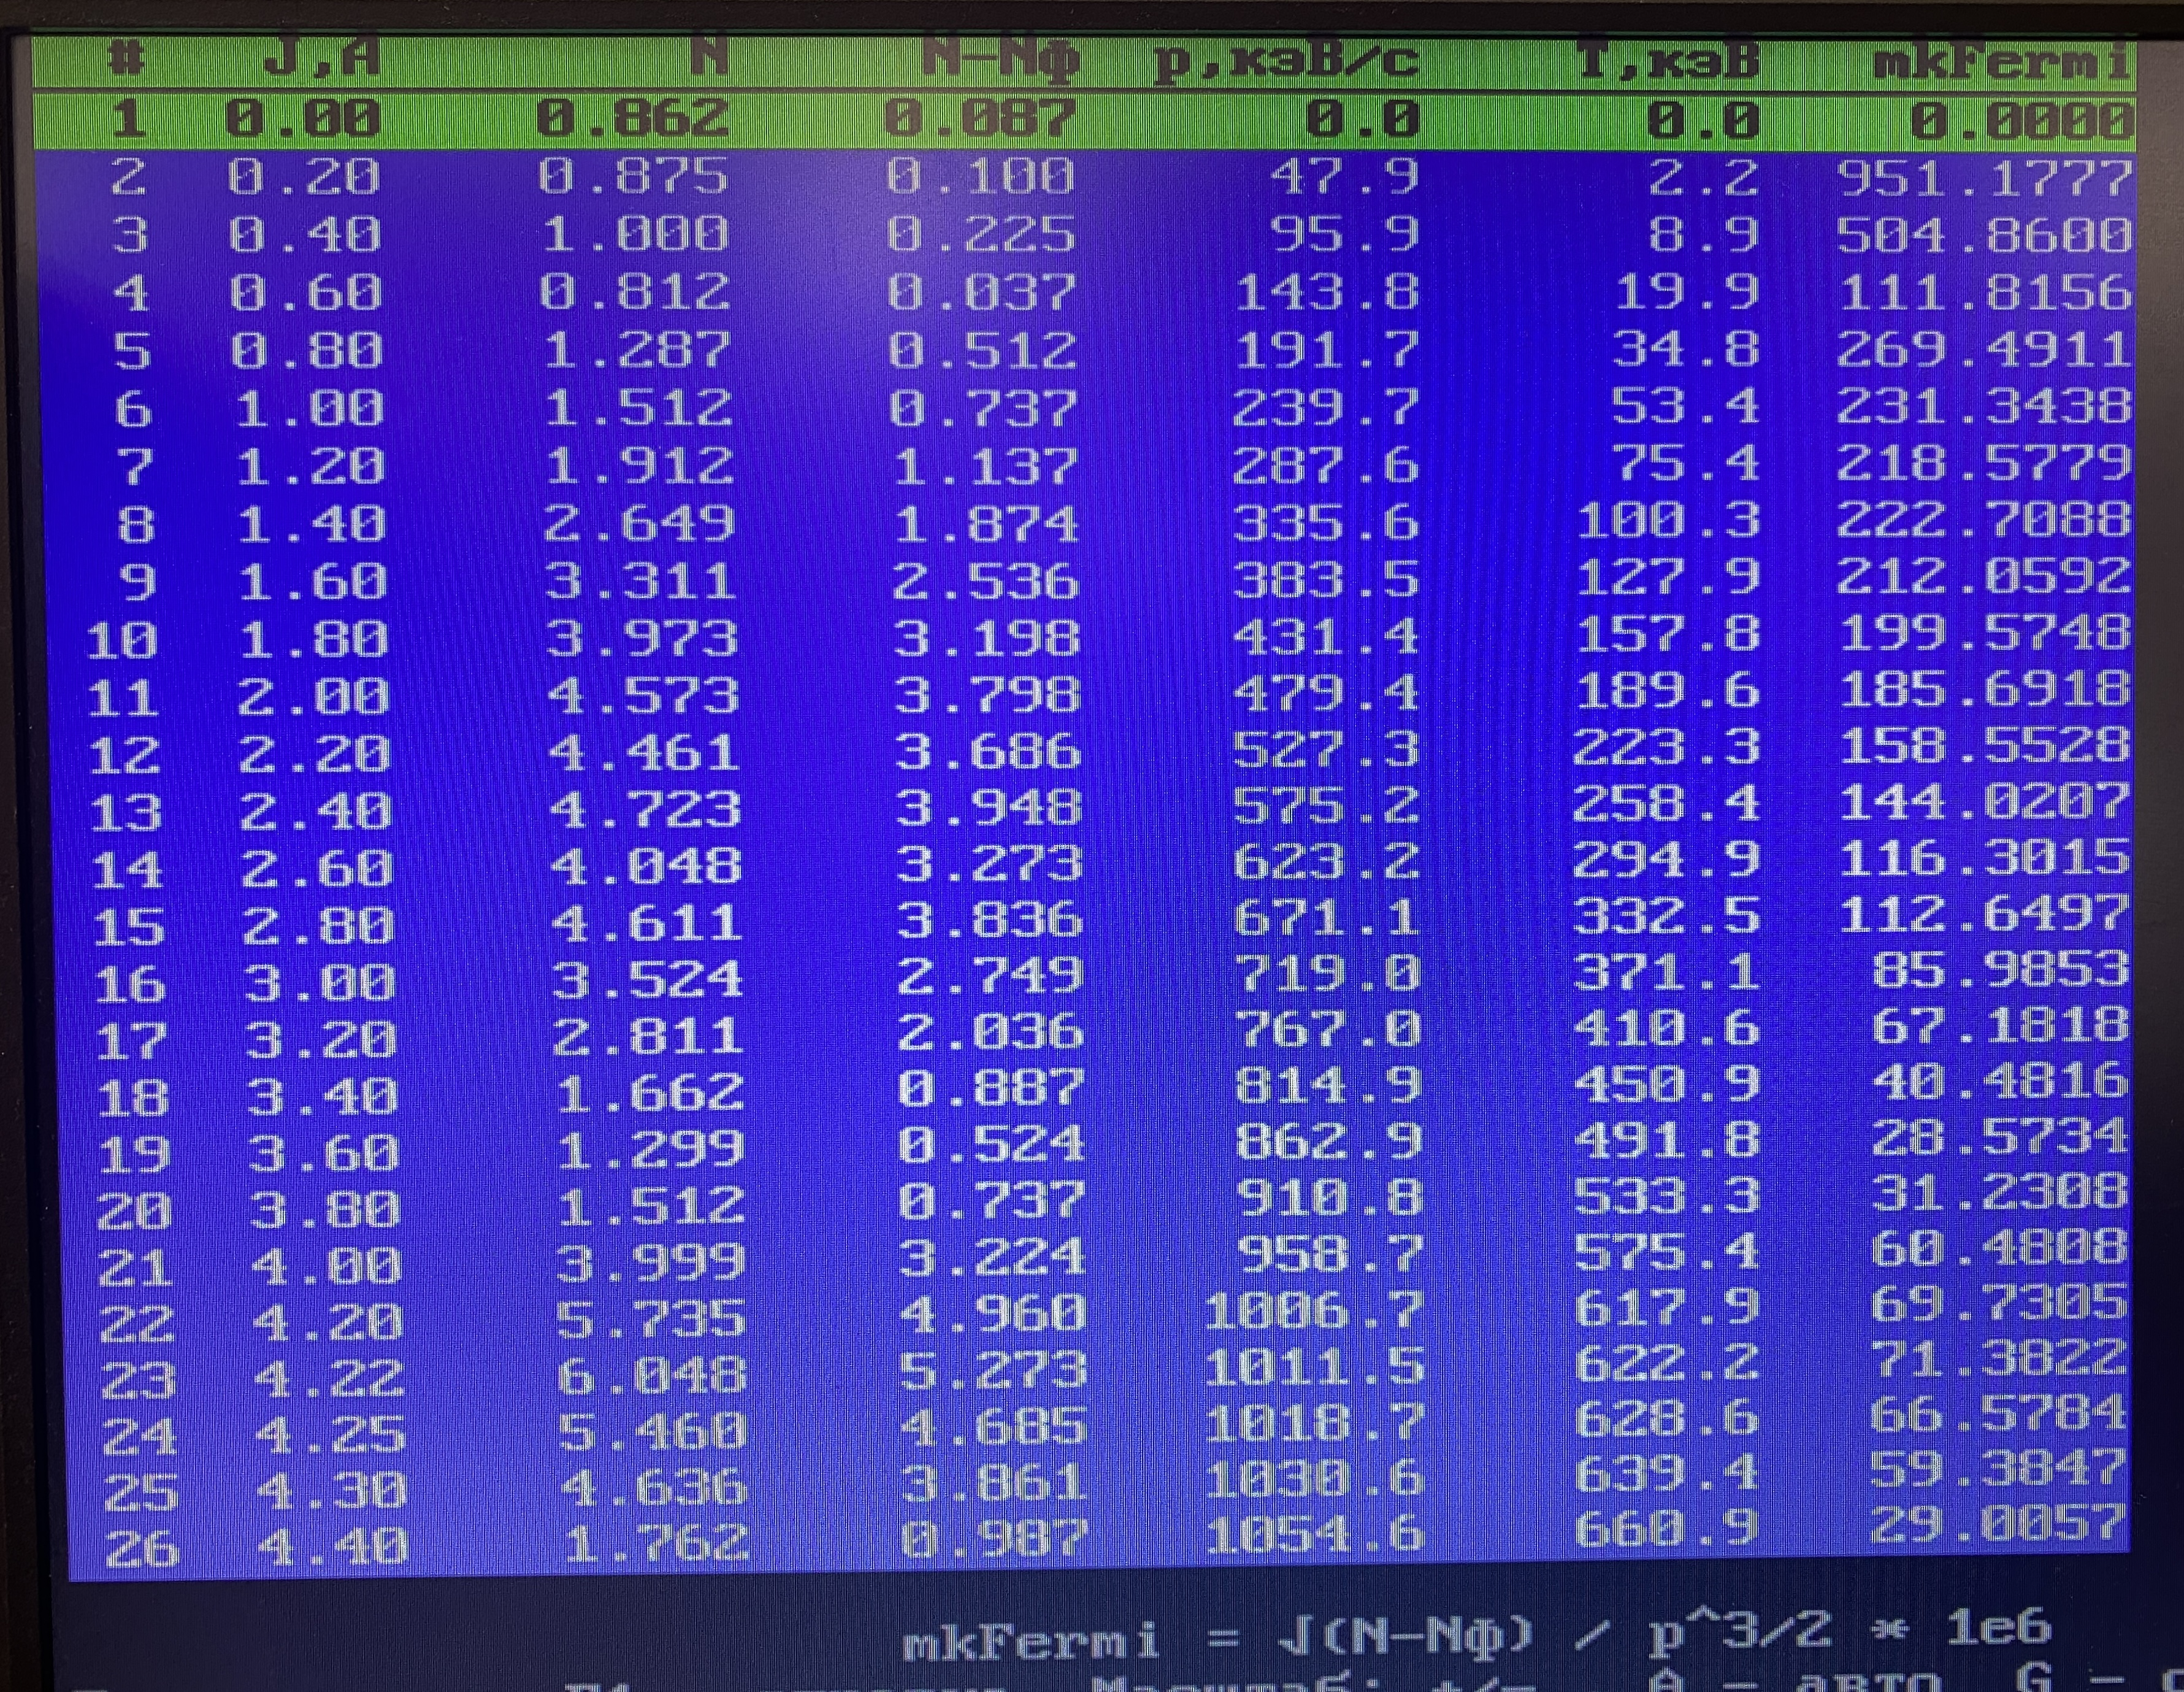
\includegraphics[width=1\textwidth]{tabl1.jpg}
    \caption{Полученные данные}
    \label{fig:tabl1}
\end{figure}

\begin{figure}[H]
    \centering
    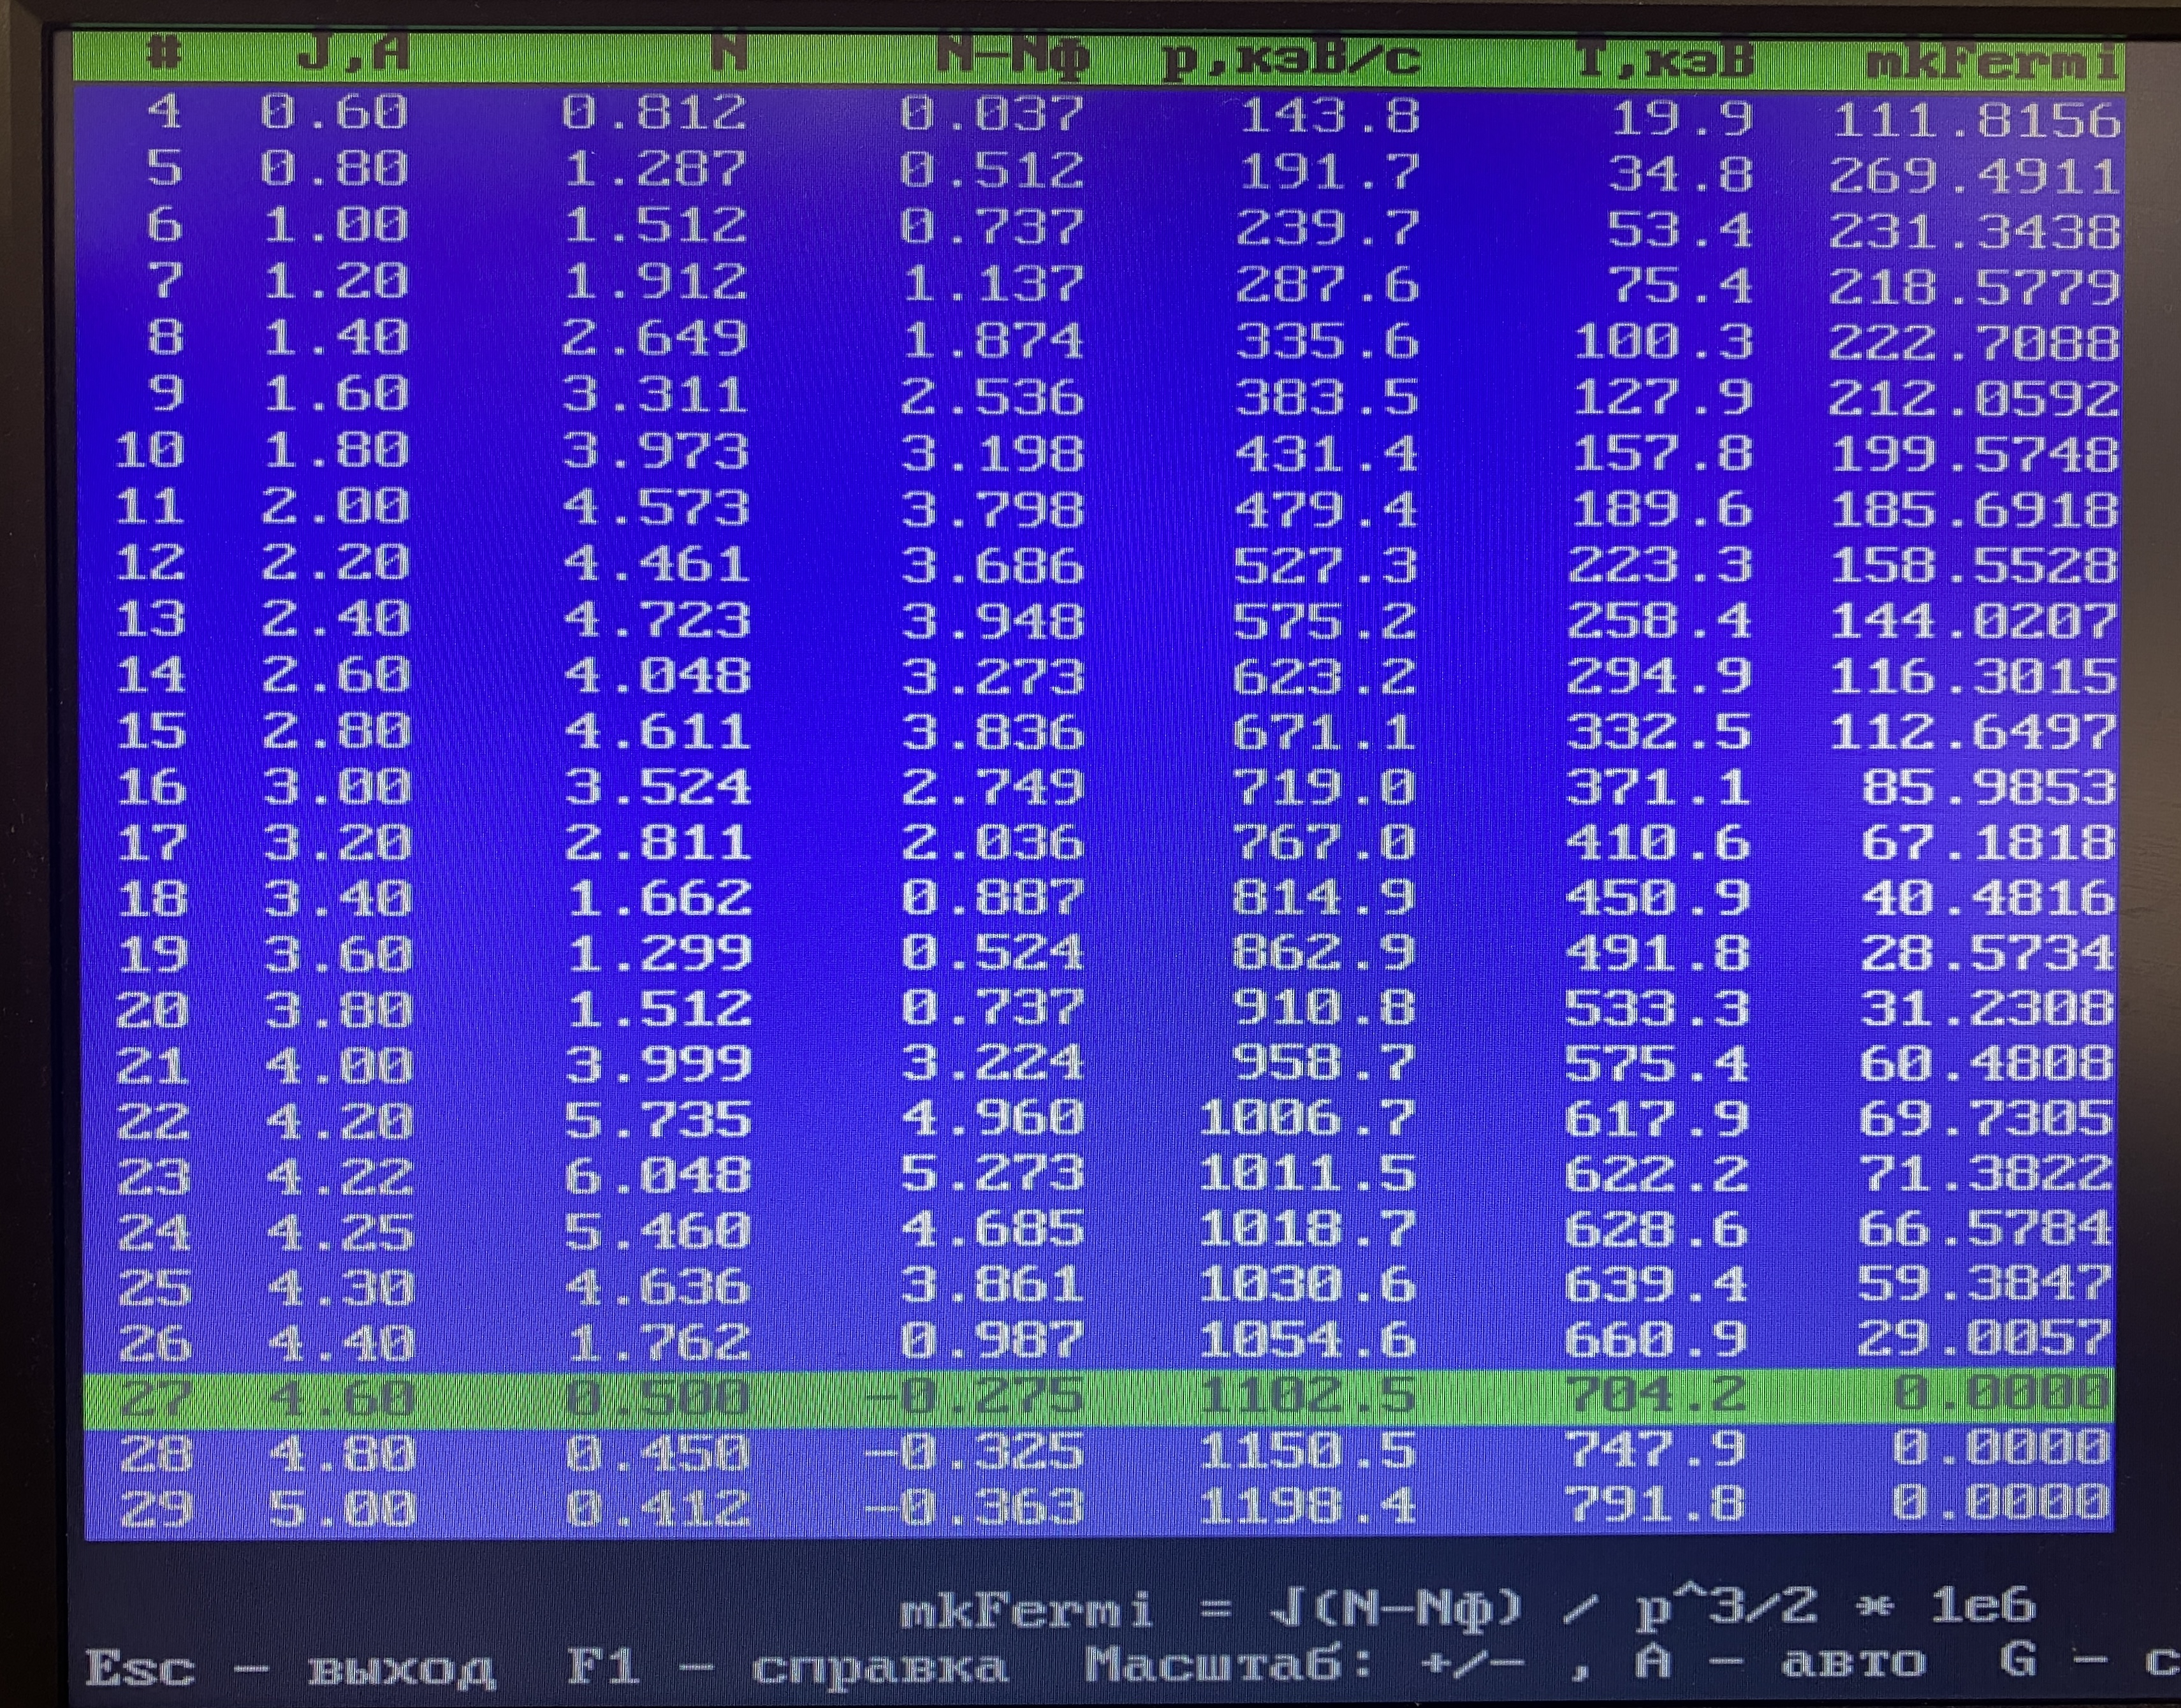
\includegraphics[width=1\textwidth]{tabl2.jpg}
    \caption{Полученные данные}
    \label{fig:tabl2}
\end{figure}
Приведем график $N - N_{\text{ф.}} = f(T)$
\begin{figure}[H]
    \centering
    \includegraphics[width=1\textwidth]{NbyT.jpg}
    \caption{График зависимости $N - N_{\text{ф.}} = f(T)$}
    \label{fig:NbyT}
\end{figure}

Конверсионный пик отсюда происходит при $I = 4.22 \ A$. Отсюда по формуле 7, полагая $p = 624 \text{ КэВ}$:
\begin{equation}
	k = \frac{624 \text{ КэВ}}{4.22 A} \approx 148 \frac{\text{ КэВ}}{A}
\end{equation}
здесь k - в единицах скорости света.

Теперь подставим значения $W(p_e)$ в (3). Сокращая обе части на $\Delta p_e$ имеем:
\begin{equation}
	\frac{\sqrt{N(p)}}{p^{3/2}} \propto T_{max} - T
\end{equation}
Такие график носит название графиков Ферми. Экстраполируя линейную часть к оси абсцисс, можно найти $T_{max} = 545 \text{ КэВ}$



\section{Выводы}


\end{document}